\section{Model Simulation} \label{sec:CombinedModel}
The found models, i.e. the attitude and translational model of the system, are presented with the constituted non-linear equations followed by the same equations linearized. Hereafter, to give a better overview, two block diagrams illustrating the linearized equations are displayed. In the last part of the section the two models are simulated, this aims to analyze the angular and translational behavior. The simulation is also used to see if the linear approximation of the equations give a valid result compared to the non-linear equations.

\subsection{Attitude Model Equations}
\begin{itemize}
	\item Model equations
	\begin{align}
		J_x \ddot{\phi}&=k_{\mathrm{th}} (\omega^2_4-\omega^2_2)  L\label{eq:AngleEqVelocitiescombined1}\\
		J_y \ddot{\theta}&=k_{\mathrm{th}} (\omega^2_1-\omega^2_3)  L\label{eq:AngleEqVelocitiescombined2}\\
		J_z \ddot{\psi}&=k_d (\omega^2_1-\omega^2_2+\omega^2_3-\omega^2_4)
		\label{eq:AngleEqVelocitiescombined3}
	\end{align}
	\item Linearized model equations
\begin{flalign}
	J_x \Delta\ddot{\phi}   &= 2 k_{\mathrm{th}} L {\overline{\omega}_4} \Delta \omega_4 - 2 k_{\mathrm{th}} L {\overline{\omega}_2} \Delta \omega_2  \label{eq:AngleLincombined1}\\
	J_y \Delta\ddot{\theta} &= 2 k_{\mathrm{th}} L \overline{\omega}_1 \Delta \omega_1 - 2 k_{\mathrm{th}} L \overline{\omega}_3 \Delta \omega_3  \label{eq:AngleLincombined2}\\
	J_z \Delta\ddot{\psi}   &= 2 k_{\mathrm{d}} {\overline{\omega}_1} \Delta \omega_1 - 2 k_{\mathrm{d}} {\overline{\omega}_2} \Delta \omega_2 + 2 k_{\mathrm{d}} {\overline{\omega}_3} \Delta \omega_3 - 2 k_{\mathrm{d}} {\overline{\omega}_4} \Delta \omega_4  \label{eq:AngleLincombined3}
	\end{flalign}
\end{itemize}
%
\subsection{Translational Model Equations}
\begin{itemize}
	\item Model equations
	\begin{flalign}
    m \ddot{x}_{\mathrm{I}} &= -k_{\mathrm{th}} ({\omega_1}^2+{\omega_2}^2+{\omega_3}^2+{\omega_4}^2) (\cos\phi \sin\theta \cos\psi + \sin\phi \sin\psi) \label{eq:AccelerationEqInertialVelocitiescombined1} \\
    m \ddot{y}_{\mathrm{I}} &= -k_{\mathrm{th}} ({\omega_1}^2+{\omega_2}^2+{\omega_3}^2+{\omega_4}^2) (\cos\phi \sin\theta \sin\psi - \sin\phi \cos\psi) \label{eq:AccelerationEqInertialVelocitiescombined2}\\
    m \ddot{z}_{\mathrm{I}} &= F_g-k_{\mathrm{th}}\ ({\omega_1}^2+{\omega_2}^2+{\omega_3}^2+{\omega_4}^2) \cos\phi \cos\theta \label{eq:AccelerationEqInertialVelocitiescombined3}
	\end{flalign}
	\item Linearized model equations 
	\begin{flalign}
			m \Delta\ddot{x}_{\mathrm{I}} &= -k_{\mathrm{th}} ({\overline{\omega}_1}^2+{\overline{\omega}_2}^2+{\overline{\omega}_3}^2+{\overline{\omega}_4}^2)  \Delta\theta \\
			m \Delta\ddot{y}_{\mathrm{I}} &=  k_{\mathrm{th}} ({\overline{\omega}_1}^2+{\overline{\omega}_2}^2+{\overline{\omega}_3}^2+{\overline{\omega}_4}^2) \Delta\phi \\
			m \Delta\ddot{z}_{\mathrm{I}} &= -2 k_{\mathrm{th}} \overline{\omega}_1 \Delta\omega_1 -2 k_{\mathrm{th}} \overline{\omega}_2 \Delta\omega_2 -2 k_{\mathrm{th}} \overline{\omega}_3 \Delta\omega_3-2 k_{\mathrm{th}} \overline{\omega}_4 \Delta\omega_4  \label{eq:FinalLinearEquationZ}
	\end{flalign} \label{eq:FinalLinearEquationscombined}
\end{itemize}

From now on, the linearized variables are represented without the symbol $\Delta$, to avoid excessive notation, even though they refer to changes around the linearization point.

\subsection{Linearized Block Diagrams}
The block diagrams of the linear approximated attitude and translational equations are illustrated in \autoref{fig:LinearModelBlockDiagram} and \ref{fig:TranslationalLinearModelBlockDiagram}. 
\begin{figure}[H]
	\centering
	\includegraphics[scale=0.3]{figures/LinearModelBlockDiag.pdf}
	\caption{A block diagram of the linearized attitude model. The input are the angular velocities of the four motors and the output are the three angles roll, pitch and yaw.}
	\label{fig:LinearModelBlockDiagram}
\end{figure}
\begin{figure}[H]
	\centering
	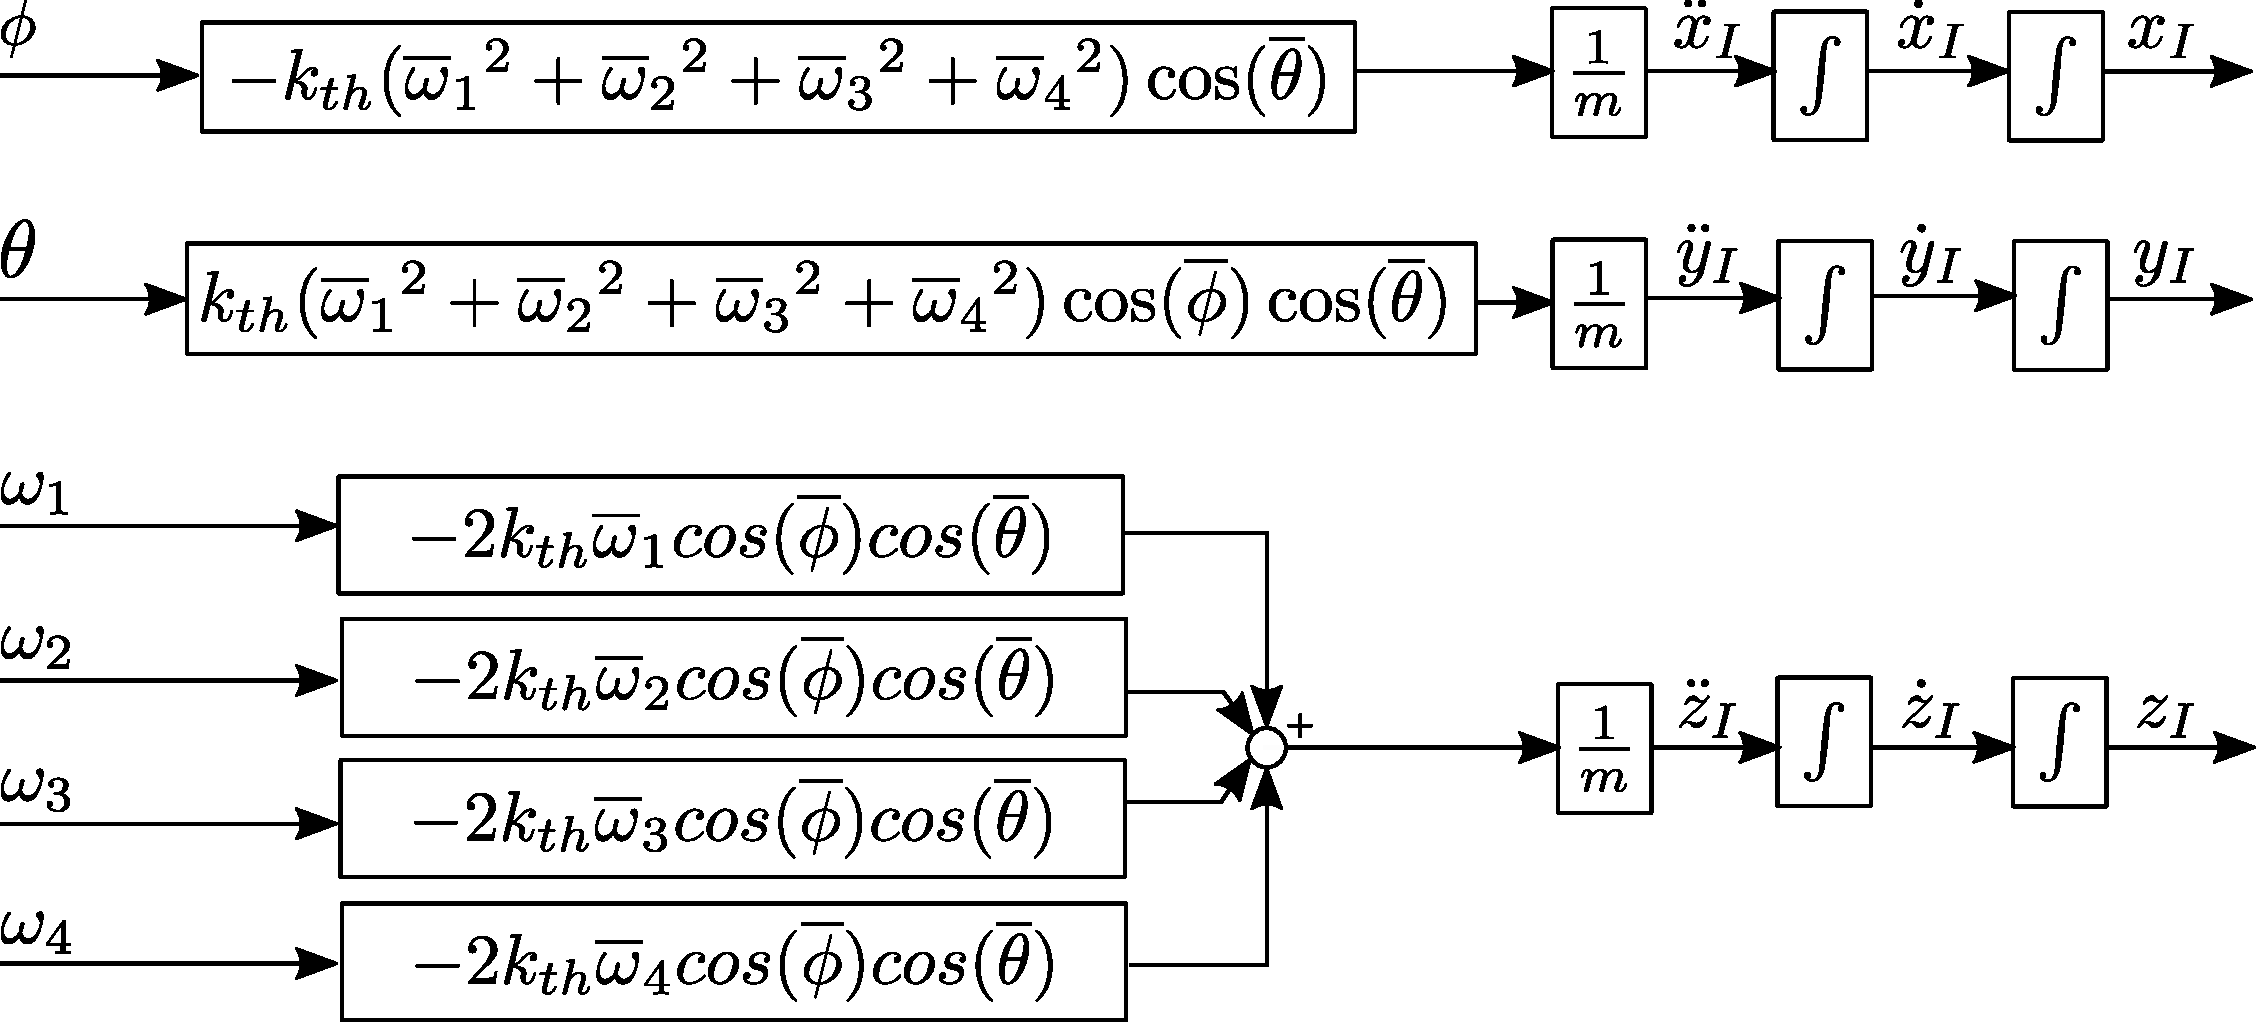
\includegraphics[scale=0.3]{figures/TranslationalLinearModelBlockDiagram.pdf}
	\caption{A block diagram of the linearized translational model. The input are the angular velocities of the four motors and the output are the three positions in $x_{\mathrm{I}}$, $y_{\mathrm{I}}$ and $z_{\mathrm{I}}$.}
	\label{fig:TranslationalLinearModelBlockDiagram}
\end{figure}

\subsection{Simulation}
A simulation of the different models is done using Simulink. The parameters needed for the simulations, that come from the model equations, are seen in \autoref{ParametersQuadcopter}.
\begin{table}[H]
	\centering
	\begin{tabular}{|l|l|l|l|}
		\hline %------------------------------------------------------------------------------------------------
		\textbf{Parameter Name}         &\textbf{Symbol} &\textbf{Value}          &\textbf{Units}             \\
		\hline %------------------------------------------------------------------------------------------------
		Mass of the quadcopter          & $m$            & 0.996             & \si{kg}                   \\
		\hline %------------------------------------------------------------------------------------------------
    Length of quadcopter arm        & $L$            & 0.225            & \si{m}                    \\
    \hline %------------------------------------------------------------------------------------------------
		Moment of inertia around $x_{\mathrm{B}}$ axis & $J_x$          & 0.01073           & \si{kg\ m^2}              \\
		\hline %------------------------------------------------------------------------------------------------
		Moment of inertia around $y_{\mathrm{B}}$ axis & $J_y$          & 0.01073           & \si{kg\ m^2}              \\
		\hline %------------------------------------------------------------------------------------------------
		Moment of inertia around $z_{\mathrm{B}}$ axis & $J_z$          & 0.0208           & \si{kg\ m^2}              \\
		\hline %------------------------------------------------------------------------------------------------
		Thrust force coefficient        & $k_{\mathrm{th}}$       & 1.32922 10$^{-5}$  & \si{N\ s^2\ rad^{-2}}     \\
		\hline %------------------------------------------------------------------------------------------------
		Drag torque coefficient         & $k_{\mathrm{d}}$        & 9.39741\ 10$^{-7}$  & \si{N\ m\  s^2\ rad^{-2}} \\
		\hline %------------------------------------------------------------------------------------------------
	\end{tabular}
	\caption{Parameters used in the simulation of the model.}
	\label{ParametersQuadcopter}
\end{table}\vspace{-18pt}

The mass of the quadcopter and the arm length are measured directly on the system. The three inertias are calculated analytically by dividing the quadcopter into different bodies for which the inertia is known, see \autoref{app:Inertia}. Finally, the thrust and drag coefficients are found by measuring the output force and torque when turning the propeller at a known speed, see \autoref{app:ThrustTest} and \ref{app:TorqueTest}.

\subsubsection{Attitude Model Simulations}
The angular behavior of the model is analyzed, where the input to the system are the four motor velocities. They are defined such that the response of the model is predictable and the performance can be evaluated.

The behavior around $x_{\mathrm{B}}$ axis is shown in \autoref{fig:rollCompModel}. 
%
\begin{figure}[H]
	\centering
	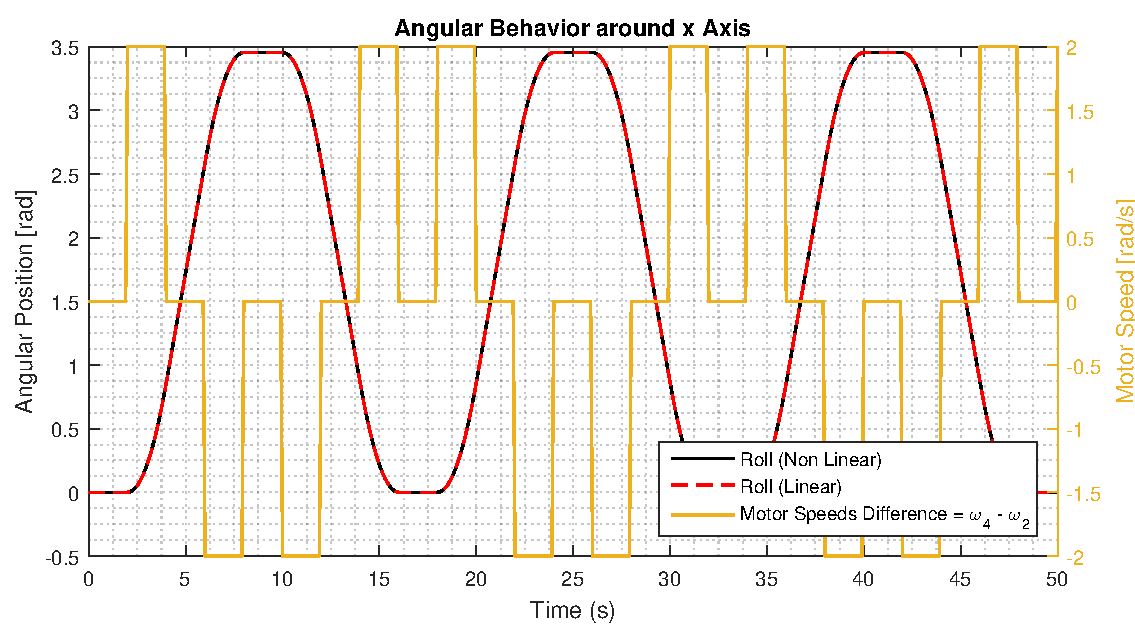
\includegraphics[scale=0.65]{figures/rollCompModel}
	\caption{Behavior of the non linear and linear models in roll angle.}
	\label{fig:rollCompModel}
\end{figure}
%
Only the speeds of motor 2 and 4 are changed as they are supposed to be the ones that affect the roll angle. It is seen that a positive difference in the rotational speeds of these motors generates a positive acceleration in the roll direction, which is consistent with \autoref{eq:AngleEqVelocitiescombined1}.

It can also be observed that the linear approximation of the equations yields an accurate result as the two responses show no perceptible difference.

\begin{figure}[H]
	\centering
	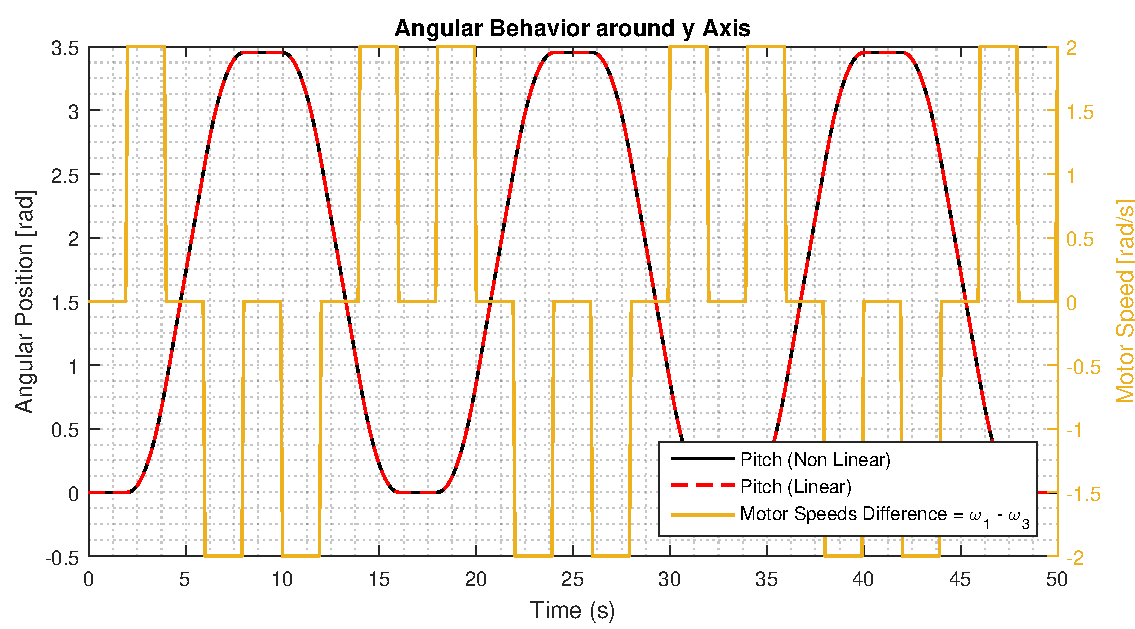
\includegraphics[scale=0.65]{figures/pitchCompModel}
	\caption{Behavior of the non linear and linear models in pitch angle.}
	\label{fig:pitchCompModel}
\end{figure}
%
The behavior around the $y_{\mathrm{B}}$ axis is very similar to that of the roll angle, see \autoref{fig:pitchCompModel}. In this case, the motor velocities modified are those from motors 1 and 3. 
%
\autoref{eq:AngleEqVelocitiescombined2} states that a positive rotational speed difference creates a positive pitch acceleration. This is confirmed by the simulations in both models. Again, the linear approximation can be considered adequate.
The last attitude response simulated is around the $z_{\mathrm{B}}$ axis and is displayed in \autoref{fig:yawCompModel}. 
%
\begin{figure}[H]
	\centering
	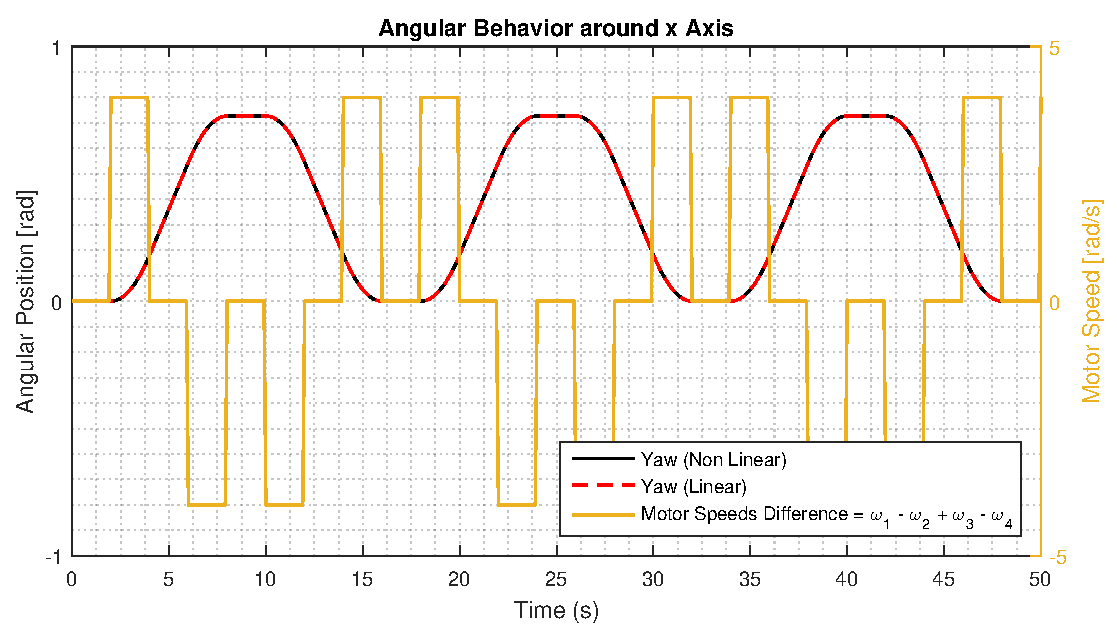
\includegraphics[scale=0.65]{figures/yawCompModel}
	\caption{Behavior of the non linear and linear models in yaw angle.}
	\label{fig:yawCompModel}
\end{figure}
In this case all motor velocities affect the yaw angle. In the simulation, velocities of motor 1 and 3 are increased while those of motor 2 and 4 are decreased and vice versa. This creates yaw accelerations according to \autoref{eq:AngleEqVelocitiescombined3}. 
The response of the model is also correct and the linear approximation is accurate.

As the linear attitude approximations are verified, the linear translational approximations are to be evaluated. 
\subsubsection{Translational Model Simulations}
The translational behavior of the model is analyzed, where the inputs are the roll and pitch angles and the addition of the four motor velocities. 

\autoref{fig:xCompModel} shows how the position in the $x_{\mathrm{I}}$ axis evolves with constant velocities of the motors and a change in the pitch angle.
\begin{figure}[H]
	\centering
	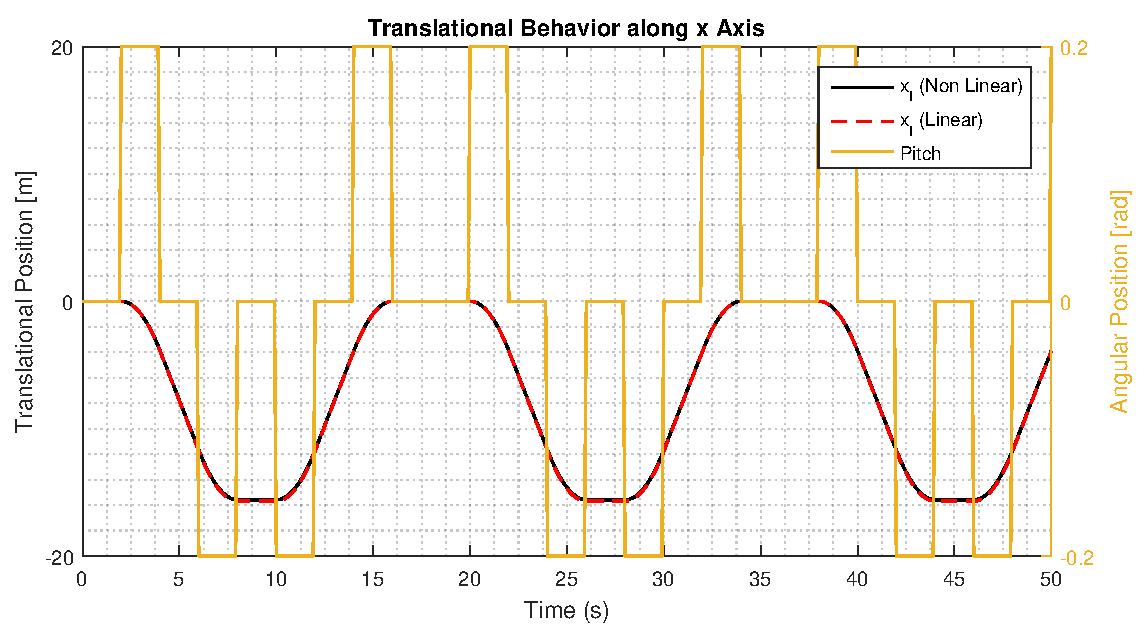
\includegraphics[scale=0.65]{figures/xCompModel}
	\caption{Behavior of the non linear and linear models along the $x_{\mathrm{I}}$ axis.}
	\label{fig:xCompModel}
\end{figure}
As expected, a negative translational acceleration is generated for a positive angle change, which drives the position to negative values. This response follows \autoref{eq:AccelerationEqInertialVelocitiescombined1}. The linear approximation is considered suitable when looking at the linear model response.
\begin{figure}[H]
	\centering
	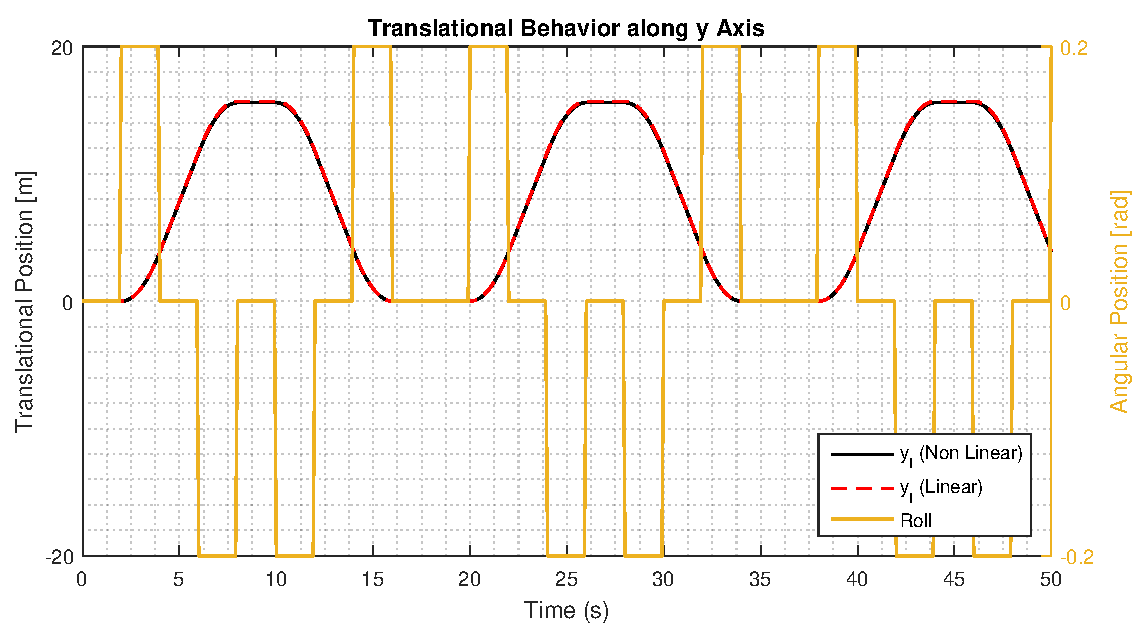
\includegraphics[scale=0.65]{figures/yCompModel}
	\caption{Behavior of the non linear and linear models along the $y_{\mathrm{I}}$ axis.}
	\label{fig:yCompModel}
\end{figure}
The response along the $y_{\mathrm{I}}$ inertial direction is depicted in \autoref{fig:yCompModel}. It is similar to that of the $x_{\mathrm{I}}$ direction but in this case a change in roll is needed to change the acceleration. Now, a positive roll angle generates a positive acceleration, as opposed to the $x_{\mathrm{I}}$ axis case. All goes in accordance with \autoref{eq:AccelerationEqInertialVelocitiescombined2}. As previously, the linear approximation performs well in the simulation.
 
\begin{figure}[H]
	\centering
	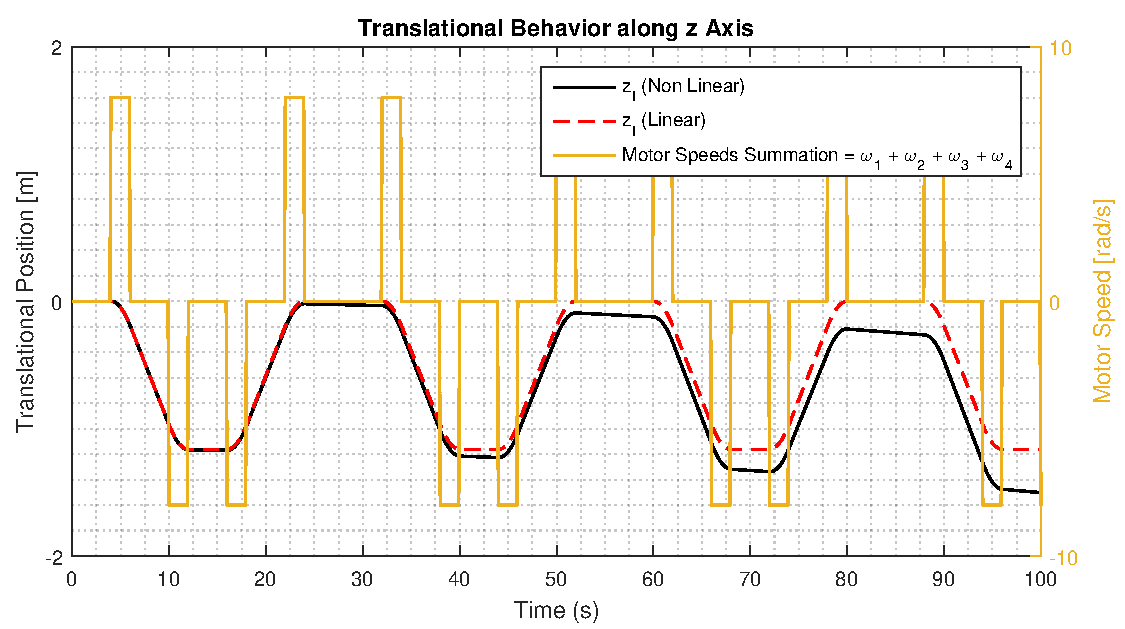
\includegraphics[scale=0.65]{figures/zCompModel}
	\caption{Behavior of the non linear and linear models along the $z_{\mathrm{I}}$ axis.}
	\label{fig:zCompModel}
\end{figure}
Finally, \autoref{fig:zCompModel} presents the behavior along the $z_{\mathrm{I}}$ axis. The pitch and roll angle are kept to zero and the summation of motor velocities are changed. For a higher sum, a more negative acceleration in the $z_{\mathrm{I}}$ axis is generated as seen in \autoref{eq:AccelerationEqInertialVelocitiescombined3} and in the simulation through the $z_{\mathrm{I}}$ position. In this case, the linear approximation of the squared velocity term in the equations creates a difference in the output $z_{\mathrm{I}}$ position between the two models that is noticeable in the graph. 
This is not a problem in the nonlinear model of the $x_{\mathrm{I}}$ and $y_{\mathrm{I}}$ translational models, as these only depend on equilibrium velocities. In the case of $x_{\mathrm{I}}$ and $y_{\mathrm{I}}$, the velocities are constant squared and not the acting variables squared, as it is for the $z_{\mathrm{I}}$ controller.

In this chapter, the attitude and translational models of the system have been derived. A linear approximation of the obtained equations are used to design the necessary controllers, see \autoref{chap:Control}.
